% Idea 3: marginal utility of modality budgets. % Idea 3: marginal utility of modality budgets. % Idea 3: marginal utility of modality budgets. % Idea 3: marginal utility of modality budgets. \input{idea3} from the midterm report.
% Needs: booktabs, cleveref, graphicx; bib entries in references_idea3.bib.
% Figures: figures/idea3_*.pdf (regenerate with `python -m src.idea3.analyze`).

\section{Idea 3: Marginal Utility of Modality Budgets}
\label{sec:idea3}

\subsection{Motivation and Initial Implementation}

Our Assignment 2 analyses suggested that image and audio contribute unequally on
OmniBench and that the imbalance flips with audio type: the raw image helped
on speech items, while on sound events audio alone beat image alone. If this
holds, a fixed input recipe wastes computation, and the cheapest way to reach
a target accuracy is to allocate visual and audio tokens \emph{per audio
type}. Idea~3 tests this premise directly by asking how much accuracy each
additional image or audio token buys, and whether the answer is stable enough
to drive a budget policy.

\paragraph{Formalization.} An item is $x=(q,O,v,a)$ with question $q$, four
options $O$, image $v$, audio $a$, and gold option $y$. A \emph{budget cell}
$b=(b_v,b_a)$ fixes the image representation $b_v\in\{0,64,256,768\}$
(maximum visual tokens; Qwen's resizer sets $\text{max\_pixels}=28^2 b_v$) and
the audio representation $b_a\in\{0,\tfrac14,\tfrac12,1\}$ (leading fraction
of the clip, at least 1\,s; 25 audio tokens/s). We add three text-surrogate
cells in which the caption and/or transcript replaces the raw modality. For a
model $f_\theta$ and option permutation $\pi$, we score
\begin{equation}
s(x;b)=\mathbb{E}_{\pi}\big[\log p_\theta(y\mid q,O_\pi,v^{(b_v)},a^{(b_a)})\big],
\end{equation}
where the expectation is over three option orders (identity and two seeded
shuffles), which removes OmniBench's answer-position skew. We use the
continuous score $s$ rather than 0/1 accuracy because it is far less noisy on
90-item subsets; accuracy (also order-averaged) is reported alongside. The
cost $c(x;b)$ is the number of input tokens.

\emph{Modality attribution.} From the four corner cells we compute per-item
two-player Shapley values~\citep{shapley1953value,lundberg2017shap} and the
interaction term~\citep{hessel2020emap}:
\begin{align}
\phi_v(x)&=\tfrac12\big[(s_{va}-s_{a})+(s_{v}-s_{\varnothing})\big],\quad
\phi_a(x)=\tfrac12\big[(s_{va}-s_{v})+(s_{a}-s_{\varnothing})\big],\nonumber\\
I(x)&=s_{va}-s_{v}-s_{a}+s_{\varnothing},
\end{align}
where $s_{va}=s(x;768,1)$, $s_v=s(x;768,0)$, $s_a=s(x;0,1)$ and
$s_\varnothing=s(x;0,0)$. $I>0$ means the modalities are worth more together
than the sum of their solo contributions.

\emph{Marginal utility and policy.} The marginal utility of an image upgrade
is $\mathrm{MU}_v(b_v\!\to\!b_v')=\mathbb{E}[s(x;b_v',b_a)-s(x;b_v,b_a)]/
\mathbb{E}[c(x;b_v',b_a)-c(x;b_v,b_a)]$, and likewise for audio. The baseline
policy is a lookup table $\pi_\beta:\text{audio type}\to b$ that maximizes dev
accuracy subject to a relative cost budget,
\begin{equation}
\pi_\beta(t)=\arg\max_{b}\ \widehat{\mathrm{acc}}_{\text{dev}}(b\mid t)
\ \ \text{s.t.}\ \ \widehat{\mathbb{E}}_{\text{dev}}\!\left[\tfrac{c(x;b)}{c(x;768,1)}\,\middle|\,t\right]\le\beta,
\end{equation}
compared against a \emph{global} policy (one cell for all items), the full
input, an always-``D'' prior, and a per-item oracle that picks the cheapest
cell correct under all three orders.

\paragraph{Setup.} We use Qwen2.5-Omni-3B~\citep{xu2025qwen25omni} (thinker
only, single forward pass, softmax over the A--D letter logits) with the
Analysis~2 prompt. The dev set is our 90-item Analysis~2 subset; for testing
we draw a disjoint, seeded 90-item set with the same balance (30 per audio
type). Each split runs the full $4\times4$ grid plus the three surrogate
cells (dev also runs two centered-window audio ablations), i.e.\ 10{,}800
forward passes in total on one V100 (fp32, $\approx$0.4\,s/pass). The grid
corners reproduce our earlier M2 Max bf16 run: predictions agree on 97.5\% of
the 1{,}890 shared passes. Budgets map to 56/240/694 visual tokens on average
because of aspect-ratio rounding.

\subsection{Results and Discussion}

\begin{table}[t]
\caption{Test accuracy (\%, mean over 3 option orders; 30 items per audio type)
and mean input tokens for selected budget cells; dev accuracy (all types) in the
last column. $b_v$ = max image tokens, $b_a$ = audio fraction.}
\label{tab:idea3-grid}
\centering\small
\setlength{\tabcolsep}{3pt}
\begin{tabular}{lcccccc}
\toprule
Cell $(b_v,b_a)$ & Speech & Sound & Music & All & Tok. & Dev \\
\midrule
$(0,0)$ question only  & 21.1 & 24.4 & 41.1 & 28.9 &  127 & 31.1 \\
$(0,1)$ audio only     & 25.6 & 26.7 & 44.4 & 32.2 &  408 & 43.7 \\
$(768,0)$ image only   & 35.6 & 21.1 & 44.4 & 33.7 &  824 & 38.1 \\
$(64,1)$               & 46.7 & \textbf{45.6} & 48.9 & 47.0 &  466 & 44.4 \\
$(256,1)$              & 52.2 & 41.1 & 48.9 & 47.4 &  650 & 45.2 \\
$(768,1)$ full input   & \textbf{53.3} & 43.3 & 53.3 & 50.0 & 1104 & 45.2 \\
Caption+transcript     & 42.2 & 33.3 & 54.4 & 43.3 &  364 & 47.8 \\
Image+transcript       & \textbf{53.3} & 44.4 & \textbf{57.8} & \textbf{51.9} &  849 & \textbf{51.1} \\
\bottomrule
\end{tabular}
\end{table}

\begin{figure*}[t]
\centering
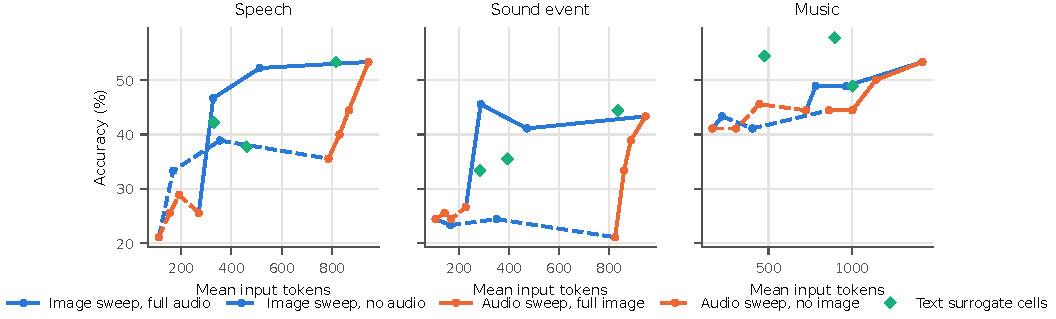
\includegraphics[width=\textwidth]{figures/idea3_marginal_curves_test.pdf}
\caption{Test accuracy vs.\ mean input tokens along each budget sweep. Blue:
image budget $0\!\to\!64\!\to\!256\!\to\!768$ tokens with full (solid) or no
(dashed) audio; orange: audio fraction $0\!\to\!\tfrac14\!\to\!\tfrac12\!\to\!1$
with full (solid) or no (dashed) image. Most of the image's value arrives in the
first 64 tokens, and only when audio is present.}
\label{fig:idea3-curves}
\end{figure*}

\paragraph{Image tokens saturate early.} The marginal utility of visual tokens
is concentrated in the first 64 (\cref{tab:idea3-grid,fig:idea3-curves}). With
full audio, a 64-token image reaches 47.0\% on test vs.\ 50.0\% for the
768-token image (paired difference $-3.0$, bootstrap 95\% CI $[-8.5,2.6]$) at
42\% of the input tokens; on dev the gap is $-0.7$ $[-7.0,5.2]$. Going from no
image to 64 tokens, by contrast, adds $+14.8$ points on test ($[7.0,23.0]$).
Audio length matters less than expected: keeping the first half of the clip
is indistinguishable from the full clip (audio only: $-0.7$ dev, $+0.7$ test).

\begin{figure}[t]
\centering
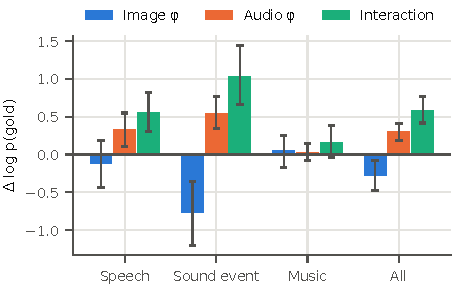
\includegraphics[width=\columnwidth]{figures/idea3_shapley.pdf}
\caption{Per-item Shapley values and interaction on $s=\log p(\text{gold})$,
dev and test pooled ($n{=}180$; bootstrap 95\% CI). Alone, the image
\emph{lowers} the gold-answer probability on sound events; together with audio,
the two modalities are strongly super-additive.}
\label{fig:idea3-shapley}
\end{figure}

\paragraph{Contributions are not additive.} \Cref{fig:idea3-shapley} shows
the attribution. On sound events the image's Shapley value is negative on
both splits (test $\phi_v=-0.74$ $[-1.38,-0.10]$; dev $-0.79$
$[-1.37,-0.25]$), audio's is positive (test $+0.52$ $[0.23,0.85]$), and the
interaction is large (test $I=+1.28$ $[0.73,1.88]$; all types $+0.60$
$[0.36,0.85]$, dev $+0.57$). The image alone does not merely fail to help: it
makes the model \emph{confidently wrong}. With image only, 36\% (dev) and 37\%
(test) of sound-event predictions are wrong with probability $>0.9$, vs.\
10--13\% with audio only. Because $I\gg0$, the utility of image tokens
depends on whether audio is present, so budgets cannot be chosen one modality
at a time. This finding replicates on held-out data; the accuracy-level
patterns we reported in Assignment~2 (e.g.\ ``audio alone beats image alone on
sound events'') hold on test as well, but other accuracy differences flip
between splits.

\begin{table}[t]
\caption{Budget policies selected on dev and scored on test. Cost is input
tokens relative to the full input. Per-type policies pick one cell per audio
type.}
\label{tab:idea3-policies}
\centering\small
\setlength{\tabcolsep}{3pt}
\begin{tabular}{llcc}
\toprule
Policy & Cells (speech / sound / music) & Acc. & Cost \\
\midrule
Always ``D''         & --                                 & 25.2 & -- \\
Full input           & $(768,1)$                          & 50.0 & 1.00 \\
Global, $\beta{=}.4$ & $(64,1)$                           & 47.0 & 0.40 \\
Per type, $\beta{=}.4$ & $(0,1)$ / $(64,1)$ / $(256,0)$    & 37.4 & 0.29 \\
Per type, $\beta{=}.6$ & $(256,1)$ / $(64,1)$ / $(256,0)$  & 46.3 & 0.38 \\
\, + surrogates, $\beta{=}.6$ & $(256,1)$ / $(64,1)$ / Cap+Tr & 50.7 & 0.40 \\
\, + surrogates, $\beta{=}.8$ & $(256,1)$ / $(64,1)$ / Img+Tr & 51.9 & 0.50 \\
Oracle (robust)      & per item                           & 52.2 & 0.22 \\
\bottomrule
\end{tabular}
\end{table}

\paragraph{Per-audio-type allocation overfits.} The premise of the baseline
is that the best cell depends on audio type. \Cref{tab:idea3-policies} shows
that a per-type table chosen on dev does \emph{worse} on test than one global
cell at the same budget: at $\beta=0.4$ it scores 37.4\% vs.\ 47.0\%
($-9.6$, $[-14.8,-4.8]$). Its music choice, image only at 256 tokens, was
the best music cell on dev (57.8\%) but scores 41.1\% on test, and its speech
choice drops the image entirely. The per-type accuracy surfaces are only
weakly stable across splits: the Spearman correlation of the 19 cell
accuracies between dev and test is 0.39--0.51 within each audio type and 0.57
overall. Thirty items per type are too few to rank 19 cells. Adding text
surrogates as candidates helps (50.7\% at 40\% cost; 51.9\% at 50\%, $+1.9$
$[-1.9,5.9]$ over the full input), mainly because image+transcript is the
strongest cell overall. The robust oracle reaches 52.2\% at 22\% of the cost,
so the remaining headroom lies in cost, not accuracy, and it is item-level, not
type-level.

\paragraph{Failure analysis.} Sorting items by the effect of adding the
image to the audio ($s_{va}-s_a$), the 25 worst items are 16 sound events, 7
speech and 2 music, mostly \emph{Action and Activity} and \emph{Story
Description} questions. They share one structure: the image shows a static
scene that matches a distractor, and only the audio reveals the event. In
item 736 (\emph{``What is this man doing?''}; audio: mechanical clicking;
image: a man holding handcuffs), audio alone puts 0.52 on the correct
\emph{``Using handcuffs''}, but the image moves 0.99 of the mass to
\emph{``Showcasing handcuffs''}, and adding the audio back leaves it at 0.99:
the image overrides the audio. In item 726 the options factor as
\{police car, fire truck\}$\times$\{honking, in motion\}. The image settles
the vehicle and the audio settles the action, but the model takes the
visually implied action (\emph{``fire truck is in motion''}). In item 842 a
cartoon dragon is drawn mid-flight while the audio is a startled scream; the
model picks \emph{``flying happily''} over \emph{``didn't fly, it fell
down''}. These are failures of cross-modal composition: the model resolves
each factor from the most salient modality instead of combining evidence. This
matches the visual dominance and modality imbalance reported for jointly
trained multimodal models~\citep{wu2022greedy,peng2022ogm}. A second, smaller
failure mode concerns truncation. We expected a centered window to preserve
short sound events better than the leading segment, but it is slightly worse
(25\%: $-1.9$, 50\%: $-3.7$ points, n.s.). Sound-event clips are short (median
3.4\,s), so the 1\,s floor makes the 25\% and 50\% cells nearly identical, and
truncation is not where the budget is lost.

\subsection{Updated Research Idea}

The midterm results change Idea~3 in three ways. (i) The relevant decision is
\emph{whether} to include a modality and at roughly what resolution, not a
fine-grained token count: 64 visual tokens and half the audio retain nearly
all of the measured utility. (ii) Audio type is too coarse a signal, and a
lookup table over it overfits; the oracle headroom is item-level. (iii)
Because $I(x)\gg0$ and the image induces confident errors, the allocator must
reason jointly about modalities and must not trust the confidence of a
single-modality pass.

For the final report we will replace the lookup table with an
\textbf{interaction-aware item-level allocator}. A cheap first pass at
$b_0=(64,\tfrac12)$ (about 30\% of the full cost) produces features
$z(x)$: the option distribution, the two disagreement statistics
$\mathrm{KL}(p_{v}\,\|\,p_{a})$ and $\mathrm{KL}(p_{va}\,\|\,p_{a})$ computed
from low-budget single-modality passes, and a question embedding. A small
regressor $g_\psi$ predicts the score gain of each upgrade, and the policy
\begin{equation}
\pi(x)=\arg\max_{b\in\mathcal{B}}\ g_\psi\big(z(x),b\big)-\lambda\,c(x;b)
\end{equation}
is trained by cross-fitting on the dev grid and evaluated on test against
this midterm's global and per-type baselines. The disagreement features target
the failure mode above: when the image and audio point to different options,
the item probably needs compositional fusion, which the full raw input
handles worst and image+transcript handles best. To keep the target from being
dominated by noise, we will train on permutation-robust correctness and
$\log p(\text{gold})$, and we will report interaction estimates under a
partial-information-decomposition view~\citep{liang2023pid} to separate
redundant from synergistic items. As a stronger point of comparison for the
resolution axis, we will also test attention-based visual token pruning in
the style of FastV~\citep{chen2024fastv} and nested visual
tokens~\citep{cai2024matryoshka} in place of resizing the image.
 from the midterm report.
% Needs: booktabs, cleveref, graphicx; bib entries in references_idea3.bib.
% Figures: figures/idea3_*.pdf (regenerate with `python -m src.idea3.analyze`).

\section{Idea 3: Marginal Utility of Modality Budgets}
\label{sec:idea3}

\subsection{Motivation and Initial Implementation}

Our Assignment 2 analyses suggested that image and audio contribute unequally on
OmniBench and that the imbalance flips with audio type: the raw image helped
on speech items, while on sound events audio alone beat image alone. If this
holds, a fixed input recipe wastes computation, and the cheapest way to reach
a target accuracy is to allocate visual and audio tokens \emph{per audio
type}. Idea~3 tests this premise directly by asking how much accuracy each
additional image or audio token buys, and whether the answer is stable enough
to drive a budget policy.

\paragraph{Formalization.} An item is $x=(q,O,v,a)$ with question $q$, four
options $O$, image $v$, audio $a$, and gold option $y$. A \emph{budget cell}
$b=(b_v,b_a)$ fixes the image representation $b_v\in\{0,64,256,768\}$
(maximum visual tokens; Qwen's resizer sets $\text{max\_pixels}=28^2 b_v$) and
the audio representation $b_a\in\{0,\tfrac14,\tfrac12,1\}$ (leading fraction
of the clip, at least 1\,s; 25 audio tokens/s). We add three text-surrogate
cells in which the caption and/or transcript replaces the raw modality. For a
model $f_\theta$ and option permutation $\pi$, we score
\begin{equation}
s(x;b)=\mathbb{E}_{\pi}\big[\log p_\theta(y\mid q,O_\pi,v^{(b_v)},a^{(b_a)})\big],
\end{equation}
where the expectation is over three option orders (identity and two seeded
shuffles), which removes OmniBench's answer-position skew. We use the
continuous score $s$ rather than 0/1 accuracy because it is far less noisy on
90-item subsets; accuracy (also order-averaged) is reported alongside. The
cost $c(x;b)$ is the number of input tokens.

\emph{Modality attribution.} From the four corner cells we compute per-item
two-player Shapley values~\citep{shapley1953value,lundberg2017shap} and the
interaction term~\citep{hessel2020emap}:
\begin{align}
\phi_v(x)&=\tfrac12\big[(s_{va}-s_{a})+(s_{v}-s_{\varnothing})\big],\quad
\phi_a(x)=\tfrac12\big[(s_{va}-s_{v})+(s_{a}-s_{\varnothing})\big],\nonumber\\
I(x)&=s_{va}-s_{v}-s_{a}+s_{\varnothing},
\end{align}
where $s_{va}=s(x;768,1)$, $s_v=s(x;768,0)$, $s_a=s(x;0,1)$ and
$s_\varnothing=s(x;0,0)$. $I>0$ means the modalities are worth more together
than the sum of their solo contributions.

\emph{Marginal utility and policy.} The marginal utility of an image upgrade
is $\mathrm{MU}_v(b_v\!\to\!b_v')=\mathbb{E}[s(x;b_v',b_a)-s(x;b_v,b_a)]/
\mathbb{E}[c(x;b_v',b_a)-c(x;b_v,b_a)]$, and likewise for audio. The baseline
policy is a lookup table $\pi_\beta:\text{audio type}\to b$ that maximizes dev
accuracy subject to a relative cost budget,
\begin{equation}
\pi_\beta(t)=\arg\max_{b}\ \widehat{\mathrm{acc}}_{\text{dev}}(b\mid t)
\ \ \text{s.t.}\ \ \widehat{\mathbb{E}}_{\text{dev}}\!\left[\tfrac{c(x;b)}{c(x;768,1)}\,\middle|\,t\right]\le\beta,
\end{equation}
compared against a \emph{global} policy (one cell for all items), the full
input, an always-``D'' prior, and a per-item oracle that picks the cheapest
cell correct under all three orders.

\paragraph{Setup.} We use Qwen2.5-Omni-3B~\citep{xu2025qwen25omni} (thinker
only, single forward pass, softmax over the A--D letter logits) with the
Analysis~2 prompt. The dev set is our 90-item Analysis~2 subset; for testing
we draw a disjoint, seeded 90-item set with the same balance (30 per audio
type). Each split runs the full $4\times4$ grid plus the three surrogate
cells (dev also runs two centered-window audio ablations), i.e.\ 10{,}800
forward passes in total on one V100 (fp32, $\approx$0.4\,s/pass). The grid
corners reproduce our earlier M2 Max bf16 run: predictions agree on 97.5\% of
the 1{,}890 shared passes. Budgets map to 56/240/694 visual tokens on average
because of aspect-ratio rounding.

\subsection{Results and Discussion}

\begin{table}[t]
\caption{Test accuracy (\%, mean over 3 option orders; 30 items per audio type)
and mean input tokens for selected budget cells; dev accuracy (all types) in the
last column. $b_v$ = max image tokens, $b_a$ = audio fraction.}
\label{tab:idea3-grid}
\centering\small
\setlength{\tabcolsep}{3pt}
\begin{tabular}{lcccccc}
\toprule
Cell $(b_v,b_a)$ & Speech & Sound & Music & All & Tok. & Dev \\
\midrule
$(0,0)$ question only  & 21.1 & 24.4 & 41.1 & 28.9 &  127 & 31.1 \\
$(0,1)$ audio only     & 25.6 & 26.7 & 44.4 & 32.2 &  408 & 43.7 \\
$(768,0)$ image only   & 35.6 & 21.1 & 44.4 & 33.7 &  824 & 38.1 \\
$(64,1)$               & 46.7 & \textbf{45.6} & 48.9 & 47.0 &  466 & 44.4 \\
$(256,1)$              & 52.2 & 41.1 & 48.9 & 47.4 &  650 & 45.2 \\
$(768,1)$ full input   & \textbf{53.3} & 43.3 & 53.3 & 50.0 & 1104 & 45.2 \\
Caption+transcript     & 42.2 & 33.3 & 54.4 & 43.3 &  364 & 47.8 \\
Image+transcript       & \textbf{53.3} & 44.4 & \textbf{57.8} & \textbf{51.9} &  849 & \textbf{51.1} \\
\bottomrule
\end{tabular}
\end{table}

\begin{figure*}[t]
\centering
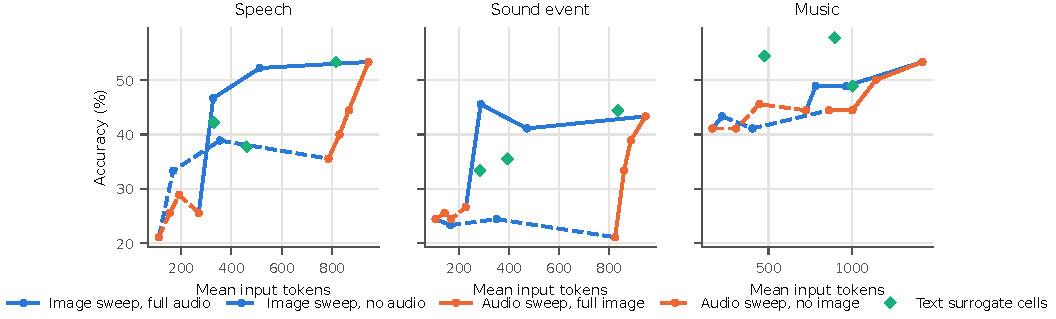
\includegraphics[width=\textwidth]{figures/idea3_marginal_curves_test.pdf}
\caption{Test accuracy vs.\ mean input tokens along each budget sweep. Blue:
image budget $0\!\to\!64\!\to\!256\!\to\!768$ tokens with full (solid) or no
(dashed) audio; orange: audio fraction $0\!\to\!\tfrac14\!\to\!\tfrac12\!\to\!1$
with full (solid) or no (dashed) image. Most of the image's value arrives in the
first 64 tokens, and only when audio is present.}
\label{fig:idea3-curves}
\end{figure*}

\paragraph{Image tokens saturate early.} The marginal utility of visual tokens
is concentrated in the first 64 (\cref{tab:idea3-grid,fig:idea3-curves}). With
full audio, a 64-token image reaches 47.0\% on test vs.\ 50.0\% for the
768-token image (paired difference $-3.0$, bootstrap 95\% CI $[-8.5,2.6]$) at
42\% of the input tokens; on dev the gap is $-0.7$ $[-7.0,5.2]$. Going from no
image to 64 tokens, by contrast, adds $+14.8$ points on test ($[7.0,23.0]$).
Audio length matters less than expected: keeping the first half of the clip
is indistinguishable from the full clip (audio only: $-0.7$ dev, $+0.7$ test).

\begin{figure}[t]
\centering
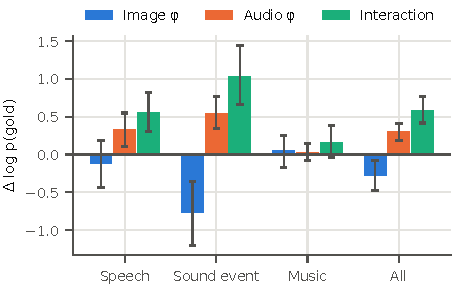
\includegraphics[width=\columnwidth]{figures/idea3_shapley.pdf}
\caption{Per-item Shapley values and interaction on $s=\log p(\text{gold})$,
dev and test pooled ($n{=}180$; bootstrap 95\% CI). Alone, the image
\emph{lowers} the gold-answer probability on sound events; together with audio,
the two modalities are strongly super-additive.}
\label{fig:idea3-shapley}
\end{figure}

\paragraph{Contributions are not additive.} \Cref{fig:idea3-shapley} shows
the attribution. On sound events the image's Shapley value is negative on
both splits (test $\phi_v=-0.74$ $[-1.38,-0.10]$; dev $-0.79$
$[-1.37,-0.25]$), audio's is positive (test $+0.52$ $[0.23,0.85]$), and the
interaction is large (test $I=+1.28$ $[0.73,1.88]$; all types $+0.60$
$[0.36,0.85]$, dev $+0.57$). The image alone does not merely fail to help: it
makes the model \emph{confidently wrong}. With image only, 36\% (dev) and 37\%
(test) of sound-event predictions are wrong with probability $>0.9$, vs.\
10--13\% with audio only. Because $I\gg0$, the utility of image tokens
depends on whether audio is present, so budgets cannot be chosen one modality
at a time. This finding replicates on held-out data; the accuracy-level
patterns we reported in Assignment~2 (e.g.\ ``audio alone beats image alone on
sound events'') hold on test as well, but other accuracy differences flip
between splits.

\begin{table}[t]
\caption{Budget policies selected on dev and scored on test. Cost is input
tokens relative to the full input. Per-type policies pick one cell per audio
type.}
\label{tab:idea3-policies}
\centering\small
\setlength{\tabcolsep}{3pt}
\begin{tabular}{llcc}
\toprule
Policy & Cells (speech / sound / music) & Acc. & Cost \\
\midrule
Always ``D''         & --                                 & 25.2 & -- \\
Full input           & $(768,1)$                          & 50.0 & 1.00 \\
Global, $\beta{=}.4$ & $(64,1)$                           & 47.0 & 0.40 \\
Per type, $\beta{=}.4$ & $(0,1)$ / $(64,1)$ / $(256,0)$    & 37.4 & 0.29 \\
Per type, $\beta{=}.6$ & $(256,1)$ / $(64,1)$ / $(256,0)$  & 46.3 & 0.38 \\
\, + surrogates, $\beta{=}.6$ & $(256,1)$ / $(64,1)$ / Cap+Tr & 50.7 & 0.40 \\
\, + surrogates, $\beta{=}.8$ & $(256,1)$ / $(64,1)$ / Img+Tr & 51.9 & 0.50 \\
Oracle (robust)      & per item                           & 52.2 & 0.22 \\
\bottomrule
\end{tabular}
\end{table}

\paragraph{Per-audio-type allocation overfits.} The premise of the baseline
is that the best cell depends on audio type. \Cref{tab:idea3-policies} shows
that a per-type table chosen on dev does \emph{worse} on test than one global
cell at the same budget: at $\beta=0.4$ it scores 37.4\% vs.\ 47.0\%
($-9.6$, $[-14.8,-4.8]$). Its music choice, image only at 256 tokens, was
the best music cell on dev (57.8\%) but scores 41.1\% on test, and its speech
choice drops the image entirely. The per-type accuracy surfaces are only
weakly stable across splits: the Spearman correlation of the 19 cell
accuracies between dev and test is 0.39--0.51 within each audio type and 0.57
overall. Thirty items per type are too few to rank 19 cells. Adding text
surrogates as candidates helps (50.7\% at 40\% cost; 51.9\% at 50\%, $+1.9$
$[-1.9,5.9]$ over the full input), mainly because image+transcript is the
strongest cell overall. The robust oracle reaches 52.2\% at 22\% of the cost,
so the remaining headroom lies in cost, not accuracy, and it is item-level, not
type-level.

\paragraph{Failure analysis.} Sorting items by the effect of adding the
image to the audio ($s_{va}-s_a$), the 25 worst items are 16 sound events, 7
speech and 2 music, mostly \emph{Action and Activity} and \emph{Story
Description} questions. They share one structure: the image shows a static
scene that matches a distractor, and only the audio reveals the event. In
item 736 (\emph{``What is this man doing?''}; audio: mechanical clicking;
image: a man holding handcuffs), audio alone puts 0.52 on the correct
\emph{``Using handcuffs''}, but the image moves 0.99 of the mass to
\emph{``Showcasing handcuffs''}, and adding the audio back leaves it at 0.99:
the image overrides the audio. In item 726 the options factor as
\{police car, fire truck\}$\times$\{honking, in motion\}. The image settles
the vehicle and the audio settles the action, but the model takes the
visually implied action (\emph{``fire truck is in motion''}). In item 842 a
cartoon dragon is drawn mid-flight while the audio is a startled scream; the
model picks \emph{``flying happily''} over \emph{``didn't fly, it fell
down''}. These are failures of cross-modal composition: the model resolves
each factor from the most salient modality instead of combining evidence. This
matches the visual dominance and modality imbalance reported for jointly
trained multimodal models~\citep{wu2022greedy,peng2022ogm}. A second, smaller
failure mode concerns truncation. We expected a centered window to preserve
short sound events better than the leading segment, but it is slightly worse
(25\%: $-1.9$, 50\%: $-3.7$ points, n.s.). Sound-event clips are short (median
3.4\,s), so the 1\,s floor makes the 25\% and 50\% cells nearly identical, and
truncation is not where the budget is lost.

\subsection{Updated Research Idea}

The midterm results change Idea~3 in three ways. (i) The relevant decision is
\emph{whether} to include a modality and at roughly what resolution, not a
fine-grained token count: 64 visual tokens and half the audio retain nearly
all of the measured utility. (ii) Audio type is too coarse a signal, and a
lookup table over it overfits; the oracle headroom is item-level. (iii)
Because $I(x)\gg0$ and the image induces confident errors, the allocator must
reason jointly about modalities and must not trust the confidence of a
single-modality pass.

For the final report we will replace the lookup table with an
\textbf{interaction-aware item-level allocator}. A cheap first pass at
$b_0=(64,\tfrac12)$ (about 30\% of the full cost) produces features
$z(x)$: the option distribution, the two disagreement statistics
$\mathrm{KL}(p_{v}\,\|\,p_{a})$ and $\mathrm{KL}(p_{va}\,\|\,p_{a})$ computed
from low-budget single-modality passes, and a question embedding. A small
regressor $g_\psi$ predicts the score gain of each upgrade, and the policy
\begin{equation}
\pi(x)=\arg\max_{b\in\mathcal{B}}\ g_\psi\big(z(x),b\big)-\lambda\,c(x;b)
\end{equation}
is trained by cross-fitting on the dev grid and evaluated on test against
this midterm's global and per-type baselines. The disagreement features target
the failure mode above: when the image and audio point to different options,
the item probably needs compositional fusion, which the full raw input
handles worst and image+transcript handles best. To keep the target from being
dominated by noise, we will train on permutation-robust correctness and
$\log p(\text{gold})$, and we will report interaction estimates under a
partial-information-decomposition view~\citep{liang2023pid} to separate
redundant from synergistic items. As a stronger point of comparison for the
resolution axis, we will also test attention-based visual token pruning in
the style of FastV~\citep{chen2024fastv} and nested visual
tokens~\citep{cai2024matryoshka} in place of resizing the image.
 from the midterm report.
% Needs: booktabs, cleveref, graphicx; bib entries in references_idea3.bib.
% Figures: figures/idea3_*.pdf (regenerate with `python -m src.idea3.analyze`).

\section{Idea 3: Marginal Utility of Modality Budgets}
\label{sec:idea3}

\subsection{Motivation and Initial Implementation}

Our Assignment 2 analyses suggested that image and audio contribute unequally on
OmniBench and that the imbalance flips with audio type: the raw image helped
on speech items, while on sound events audio alone beat image alone. If this
holds, a fixed input recipe wastes computation, and the cheapest way to reach
a target accuracy is to allocate visual and audio tokens \emph{per audio
type}. Idea~3 tests this premise directly by asking how much accuracy each
additional image or audio token buys, and whether the answer is stable enough
to drive a budget policy.

\paragraph{Formalization.} An item is $x=(q,O,v,a)$ with question $q$, four
options $O$, image $v$, audio $a$, and gold option $y$. A \emph{budget cell}
$b=(b_v,b_a)$ fixes the image representation $b_v\in\{0,64,256,768\}$
(maximum visual tokens; Qwen's resizer sets $\text{max\_pixels}=28^2 b_v$) and
the audio representation $b_a\in\{0,\tfrac14,\tfrac12,1\}$ (leading fraction
of the clip, at least 1\,s; 25 audio tokens/s). We add three text-surrogate
cells in which the caption and/or transcript replaces the raw modality. For a
model $f_\theta$ and option permutation $\pi$, we score
\begin{equation}
s(x;b)=\mathbb{E}_{\pi}\big[\log p_\theta(y\mid q,O_\pi,v^{(b_v)},a^{(b_a)})\big],
\end{equation}
where the expectation is over three option orders (identity and two seeded
shuffles), which removes OmniBench's answer-position skew. We use the
continuous score $s$ rather than 0/1 accuracy because it is far less noisy on
90-item subsets; accuracy (also order-averaged) is reported alongside. The
cost $c(x;b)$ is the number of input tokens.

\emph{Modality attribution.} From the four corner cells we compute per-item
two-player Shapley values~\citep{shapley1953value,lundberg2017shap} and the
interaction term~\citep{hessel2020emap}:
\begin{align}
\phi_v(x)&=\tfrac12\big[(s_{va}-s_{a})+(s_{v}-s_{\varnothing})\big],\quad
\phi_a(x)=\tfrac12\big[(s_{va}-s_{v})+(s_{a}-s_{\varnothing})\big],\nonumber\\
I(x)&=s_{va}-s_{v}-s_{a}+s_{\varnothing},
\end{align}
where $s_{va}=s(x;768,1)$, $s_v=s(x;768,0)$, $s_a=s(x;0,1)$ and
$s_\varnothing=s(x;0,0)$. $I>0$ means the modalities are worth more together
than the sum of their solo contributions.

\emph{Marginal utility and policy.} The marginal utility of an image upgrade
is $\mathrm{MU}_v(b_v\!\to\!b_v')=\mathbb{E}[s(x;b_v',b_a)-s(x;b_v,b_a)]/
\mathbb{E}[c(x;b_v',b_a)-c(x;b_v,b_a)]$, and likewise for audio. The baseline
policy is a lookup table $\pi_\beta:\text{audio type}\to b$ that maximizes dev
accuracy subject to a relative cost budget,
\begin{equation}
\pi_\beta(t)=\arg\max_{b}\ \widehat{\mathrm{acc}}_{\text{dev}}(b\mid t)
\ \ \text{s.t.}\ \ \widehat{\mathbb{E}}_{\text{dev}}\!\left[\tfrac{c(x;b)}{c(x;768,1)}\,\middle|\,t\right]\le\beta,
\end{equation}
compared against a \emph{global} policy (one cell for all items), the full
input, an always-``D'' prior, and a per-item oracle that picks the cheapest
cell correct under all three orders.

\paragraph{Setup.} We use Qwen2.5-Omni-3B~\citep{xu2025qwen25omni} (thinker
only, single forward pass, softmax over the A--D letter logits) with the
Analysis~2 prompt. The dev set is our 90-item Analysis~2 subset; for testing
we draw a disjoint, seeded 90-item set with the same balance (30 per audio
type). Each split runs the full $4\times4$ grid plus the three surrogate
cells (dev also runs two centered-window audio ablations), i.e.\ 10{,}800
forward passes in total on one V100 (fp32, $\approx$0.4\,s/pass). The grid
corners reproduce our earlier M2 Max bf16 run: predictions agree on 97.5\% of
the 1{,}890 shared passes. Budgets map to 56/240/694 visual tokens on average
because of aspect-ratio rounding.

\subsection{Results and Discussion}

\begin{table}[t]
\caption{Test accuracy (\%, mean over 3 option orders; 30 items per audio type)
and mean input tokens for selected budget cells; dev accuracy (all types) in the
last column. $b_v$ = max image tokens, $b_a$ = audio fraction.}
\label{tab:idea3-grid}
\centering\small
\setlength{\tabcolsep}{3pt}
\begin{tabular}{lcccccc}
\toprule
Cell $(b_v,b_a)$ & Speech & Sound & Music & All & Tok. & Dev \\
\midrule
$(0,0)$ question only  & 21.1 & 24.4 & 41.1 & 28.9 &  127 & 31.1 \\
$(0,1)$ audio only     & 25.6 & 26.7 & 44.4 & 32.2 &  408 & 43.7 \\
$(768,0)$ image only   & 35.6 & 21.1 & 44.4 & 33.7 &  824 & 38.1 \\
$(64,1)$               & 46.7 & \textbf{45.6} & 48.9 & 47.0 &  466 & 44.4 \\
$(256,1)$              & 52.2 & 41.1 & 48.9 & 47.4 &  650 & 45.2 \\
$(768,1)$ full input   & \textbf{53.3} & 43.3 & 53.3 & 50.0 & 1104 & 45.2 \\
Caption+transcript     & 42.2 & 33.3 & 54.4 & 43.3 &  364 & 47.8 \\
Image+transcript       & \textbf{53.3} & 44.4 & \textbf{57.8} & \textbf{51.9} &  849 & \textbf{51.1} \\
\bottomrule
\end{tabular}
\end{table}

\begin{figure*}[t]
\centering
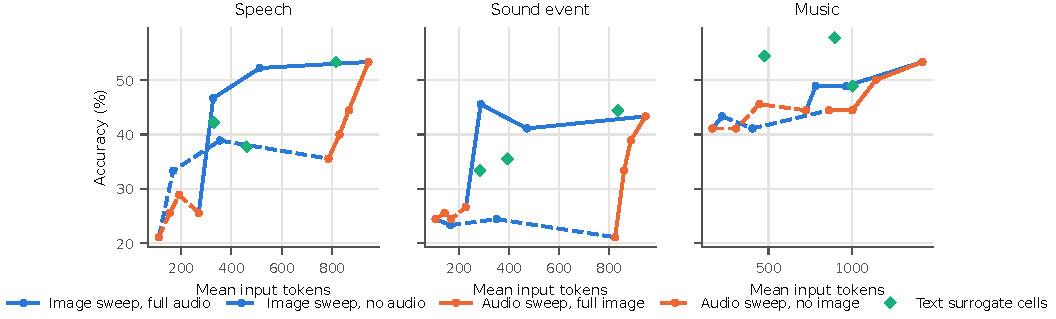
\includegraphics[width=\textwidth]{figures/idea3_marginal_curves_test.pdf}
\caption{Test accuracy vs.\ mean input tokens along each budget sweep. Blue:
image budget $0\!\to\!64\!\to\!256\!\to\!768$ tokens with full (solid) or no
(dashed) audio; orange: audio fraction $0\!\to\!\tfrac14\!\to\!\tfrac12\!\to\!1$
with full (solid) or no (dashed) image. Most of the image's value arrives in the
first 64 tokens, and only when audio is present.}
\label{fig:idea3-curves}
\end{figure*}

\paragraph{Image tokens saturate early.} The marginal utility of visual tokens
is concentrated in the first 64 (\cref{tab:idea3-grid,fig:idea3-curves}). With
full audio, a 64-token image reaches 47.0\% on test vs.\ 50.0\% for the
768-token image (paired difference $-3.0$, bootstrap 95\% CI $[-8.5,2.6]$) at
42\% of the input tokens; on dev the gap is $-0.7$ $[-7.0,5.2]$. Going from no
image to 64 tokens, by contrast, adds $+14.8$ points on test ($[7.0,23.0]$).
Audio length matters less than expected: keeping the first half of the clip
is indistinguishable from the full clip (audio only: $-0.7$ dev, $+0.7$ test).

\begin{figure}[t]
\centering
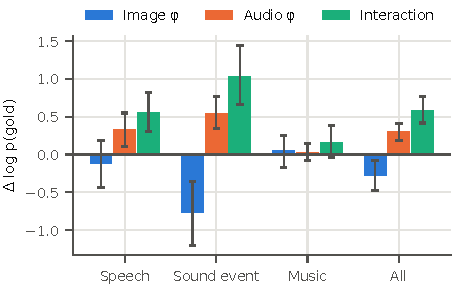
\includegraphics[width=\columnwidth]{figures/idea3_shapley.pdf}
\caption{Per-item Shapley values and interaction on $s=\log p(\text{gold})$,
dev and test pooled ($n{=}180$; bootstrap 95\% CI). Alone, the image
\emph{lowers} the gold-answer probability on sound events; together with audio,
the two modalities are strongly super-additive.}
\label{fig:idea3-shapley}
\end{figure}

\paragraph{Contributions are not additive.} \Cref{fig:idea3-shapley} shows
the attribution. On sound events the image's Shapley value is negative on
both splits (test $\phi_v=-0.74$ $[-1.38,-0.10]$; dev $-0.79$
$[-1.37,-0.25]$), audio's is positive (test $+0.52$ $[0.23,0.85]$), and the
interaction is large (test $I=+1.28$ $[0.73,1.88]$; all types $+0.60$
$[0.36,0.85]$, dev $+0.57$). The image alone does not merely fail to help: it
makes the model \emph{confidently wrong}. With image only, 36\% (dev) and 37\%
(test) of sound-event predictions are wrong with probability $>0.9$, vs.\
10--13\% with audio only. Because $I\gg0$, the utility of image tokens
depends on whether audio is present, so budgets cannot be chosen one modality
at a time. This finding replicates on held-out data; the accuracy-level
patterns we reported in Assignment~2 (e.g.\ ``audio alone beats image alone on
sound events'') hold on test as well, but other accuracy differences flip
between splits.

\begin{table}[t]
\caption{Budget policies selected on dev and scored on test. Cost is input
tokens relative to the full input. Per-type policies pick one cell per audio
type.}
\label{tab:idea3-policies}
\centering\small
\setlength{\tabcolsep}{3pt}
\begin{tabular}{llcc}
\toprule
Policy & Cells (speech / sound / music) & Acc. & Cost \\
\midrule
Always ``D''         & --                                 & 25.2 & -- \\
Full input           & $(768,1)$                          & 50.0 & 1.00 \\
Global, $\beta{=}.4$ & $(64,1)$                           & 47.0 & 0.40 \\
Per type, $\beta{=}.4$ & $(0,1)$ / $(64,1)$ / $(256,0)$    & 37.4 & 0.29 \\
Per type, $\beta{=}.6$ & $(256,1)$ / $(64,1)$ / $(256,0)$  & 46.3 & 0.38 \\
\, + surrogates, $\beta{=}.6$ & $(256,1)$ / $(64,1)$ / Cap+Tr & 50.7 & 0.40 \\
\, + surrogates, $\beta{=}.8$ & $(256,1)$ / $(64,1)$ / Img+Tr & 51.9 & 0.50 \\
Oracle (robust)      & per item                           & 52.2 & 0.22 \\
\bottomrule
\end{tabular}
\end{table}

\paragraph{Per-audio-type allocation overfits.} The premise of the baseline
is that the best cell depends on audio type. \Cref{tab:idea3-policies} shows
that a per-type table chosen on dev does \emph{worse} on test than one global
cell at the same budget: at $\beta=0.4$ it scores 37.4\% vs.\ 47.0\%
($-9.6$, $[-14.8,-4.8]$). Its music choice, image only at 256 tokens, was
the best music cell on dev (57.8\%) but scores 41.1\% on test, and its speech
choice drops the image entirely. The per-type accuracy surfaces are only
weakly stable across splits: the Spearman correlation of the 19 cell
accuracies between dev and test is 0.39--0.51 within each audio type and 0.57
overall. Thirty items per type are too few to rank 19 cells. Adding text
surrogates as candidates helps (50.7\% at 40\% cost; 51.9\% at 50\%, $+1.9$
$[-1.9,5.9]$ over the full input), mainly because image+transcript is the
strongest cell overall. The robust oracle reaches 52.2\% at 22\% of the cost,
so the remaining headroom lies in cost, not accuracy, and it is item-level, not
type-level.

\paragraph{Failure analysis.} Sorting items by the effect of adding the
image to the audio ($s_{va}-s_a$), the 25 worst items are 16 sound events, 7
speech and 2 music, mostly \emph{Action and Activity} and \emph{Story
Description} questions. They share one structure: the image shows a static
scene that matches a distractor, and only the audio reveals the event. In
item 736 (\emph{``What is this man doing?''}; audio: mechanical clicking;
image: a man holding handcuffs), audio alone puts 0.52 on the correct
\emph{``Using handcuffs''}, but the image moves 0.99 of the mass to
\emph{``Showcasing handcuffs''}, and adding the audio back leaves it at 0.99:
the image overrides the audio. In item 726 the options factor as
\{police car, fire truck\}$\times$\{honking, in motion\}. The image settles
the vehicle and the audio settles the action, but the model takes the
visually implied action (\emph{``fire truck is in motion''}). In item 842 a
cartoon dragon is drawn mid-flight while the audio is a startled scream; the
model picks \emph{``flying happily''} over \emph{``didn't fly, it fell
down''}. These are failures of cross-modal composition: the model resolves
each factor from the most salient modality instead of combining evidence. This
matches the visual dominance and modality imbalance reported for jointly
trained multimodal models~\citep{wu2022greedy,peng2022ogm}. A second, smaller
failure mode concerns truncation. We expected a centered window to preserve
short sound events better than the leading segment, but it is slightly worse
(25\%: $-1.9$, 50\%: $-3.7$ points, n.s.). Sound-event clips are short (median
3.4\,s), so the 1\,s floor makes the 25\% and 50\% cells nearly identical, and
truncation is not where the budget is lost.

\subsection{Updated Research Idea}

The midterm results change Idea~3 in three ways. (i) The relevant decision is
\emph{whether} to include a modality and at roughly what resolution, not a
fine-grained token count: 64 visual tokens and half the audio retain nearly
all of the measured utility. (ii) Audio type is too coarse a signal, and a
lookup table over it overfits; the oracle headroom is item-level. (iii)
Because $I(x)\gg0$ and the image induces confident errors, the allocator must
reason jointly about modalities and must not trust the confidence of a
single-modality pass.

For the final report we will replace the lookup table with an
\textbf{interaction-aware item-level allocator}. A cheap first pass at
$b_0=(64,\tfrac12)$ (about 30\% of the full cost) produces features
$z(x)$: the option distribution, the two disagreement statistics
$\mathrm{KL}(p_{v}\,\|\,p_{a})$ and $\mathrm{KL}(p_{va}\,\|\,p_{a})$ computed
from low-budget single-modality passes, and a question embedding. A small
regressor $g_\psi$ predicts the score gain of each upgrade, and the policy
\begin{equation}
\pi(x)=\arg\max_{b\in\mathcal{B}}\ g_\psi\big(z(x),b\big)-\lambda\,c(x;b)
\end{equation}
is trained by cross-fitting on the dev grid and evaluated on test against
this midterm's global and per-type baselines. The disagreement features target
the failure mode above: when the image and audio point to different options,
the item probably needs compositional fusion, which the full raw input
handles worst and image+transcript handles best. To keep the target from being
dominated by noise, we will train on permutation-robust correctness and
$\log p(\text{gold})$, and we will report interaction estimates under a
partial-information-decomposition view~\citep{liang2023pid} to separate
redundant from synergistic items. As a stronger point of comparison for the
resolution axis, we will also test attention-based visual token pruning in
the style of FastV~\citep{chen2024fastv} and nested visual
tokens~\citep{cai2024matryoshka} in place of resizing the image.
 from the midterm report.
% Needs: booktabs, cleveref, graphicx; bib entries in references_idea3.bib.
% Figures: figures/idea3_*.pdf (regenerate with `python -m src.idea3.analyze`).

\section{Idea 3: Marginal Utility of Modality Budgets}
\label{sec:idea3}

\subsection{Motivation and Initial Implementation}

Our Assignment 2 analyses suggested that image and audio contribute unequally on
OmniBench and that the imbalance flips with audio type: the raw image helped
on speech items, while on sound events audio alone beat image alone. If this
holds, a fixed input recipe wastes computation, and the cheapest way to reach
a target accuracy is to allocate visual and audio tokens \emph{per audio
type}. Idea~3 tests this premise directly by asking how much accuracy each
additional image or audio token buys, and whether the answer is stable enough
to drive a budget policy.

\paragraph{Formalization.} An item is $x=(q,O,v,a)$ with question $q$, four
options $O$, image $v$, audio $a$, and gold option $y$. A \emph{budget cell}
$b=(b_v,b_a)$ fixes the image representation $b_v\in\{0,64,256,768\}$
(maximum visual tokens; Qwen's resizer sets $\text{max\_pixels}=28^2 b_v$) and
the audio representation $b_a\in\{0,\tfrac14,\tfrac12,1\}$ (leading fraction
of the clip, at least 1\,s; 25 audio tokens/s). We add three text-surrogate
cells in which the caption and/or transcript replaces the raw modality. For a
model $f_\theta$ and option permutation $\pi$, we score
\begin{equation}
s(x;b)=\mathbb{E}_{\pi}\big[\log p_\theta(y\mid q,O_\pi,v^{(b_v)},a^{(b_a)})\big],
\end{equation}
where the expectation is over three option orders (identity and two seeded
shuffles), which removes OmniBench's answer-position skew. We use the
continuous score $s$ rather than 0/1 accuracy because it is far less noisy on
90-item subsets; accuracy (also order-averaged) is reported alongside. The
cost $c(x;b)$ is the number of input tokens.

\emph{Modality attribution.} From the four corner cells we compute per-item
two-player Shapley values~\citep{shapley1953value,lundberg2017shap} and the
interaction term~\citep{hessel2020emap}:
\begin{align}
\phi_v(x)&=\tfrac12\big[(s_{va}-s_{a})+(s_{v}-s_{\varnothing})\big],\quad
\phi_a(x)=\tfrac12\big[(s_{va}-s_{v})+(s_{a}-s_{\varnothing})\big],\nonumber\\
I(x)&=s_{va}-s_{v}-s_{a}+s_{\varnothing},
\end{align}
where $s_{va}=s(x;768,1)$, $s_v=s(x;768,0)$, $s_a=s(x;0,1)$ and
$s_\varnothing=s(x;0,0)$. $I>0$ means the modalities are worth more together
than the sum of their solo contributions.

\emph{Marginal utility and policy.} The marginal utility of an image upgrade
is $\mathrm{MU}_v(b_v\!\to\!b_v')=\mathbb{E}[s(x;b_v',b_a)-s(x;b_v,b_a)]/
\mathbb{E}[c(x;b_v',b_a)-c(x;b_v,b_a)]$, and likewise for audio. The baseline
policy is a lookup table $\pi_\beta:\text{audio type}\to b$ that maximizes dev
accuracy subject to a relative cost budget,
\begin{equation}
\pi_\beta(t)=\arg\max_{b}\ \widehat{\mathrm{acc}}_{\text{dev}}(b\mid t)
\ \ \text{s.t.}\ \ \widehat{\mathbb{E}}_{\text{dev}}\!\left[\tfrac{c(x;b)}{c(x;768,1)}\,\middle|\,t\right]\le\beta,
\end{equation}
compared against a \emph{global} policy (one cell for all items), the full
input, an always-``D'' prior, and a per-item oracle that picks the cheapest
cell correct under all three orders.

\paragraph{Setup.} We use Qwen2.5-Omni-3B~\citep{xu2025qwen25omni} (thinker
only, single forward pass, softmax over the A--D letter logits) with the
Analysis~2 prompt. The dev set is our 90-item Analysis~2 subset; for testing
we draw a disjoint, seeded 90-item set with the same balance (30 per audio
type). Each split runs the full $4\times4$ grid plus the three surrogate
cells (dev also runs two centered-window audio ablations), i.e.\ 10{,}800
forward passes in total on one V100 (fp32, $\approx$0.4\,s/pass). The grid
corners reproduce our earlier M2 Max bf16 run: predictions agree on 97.5\% of
the 1{,}890 shared passes. Budgets map to 56/240/694 visual tokens on average
because of aspect-ratio rounding.

\subsection{Results and Discussion}

\begin{table}[t]
\caption{Test accuracy (\%, mean over 3 option orders; 30 items per audio type)
and mean input tokens for selected budget cells; dev accuracy (all types) in the
last column. $b_v$ = max image tokens, $b_a$ = audio fraction.}
\label{tab:idea3-grid}
\centering\small
\setlength{\tabcolsep}{3pt}
\begin{tabular}{lcccccc}
\toprule
Cell $(b_v,b_a)$ & Speech & Sound & Music & All & Tok. & Dev \\
\midrule
$(0,0)$ question only  & 21.1 & 24.4 & 41.1 & 28.9 &  127 & 31.1 \\
$(0,1)$ audio only     & 25.6 & 26.7 & 44.4 & 32.2 &  408 & 43.7 \\
$(768,0)$ image only   & 35.6 & 21.1 & 44.4 & 33.7 &  824 & 38.1 \\
$(64,1)$               & 46.7 & \textbf{45.6} & 48.9 & 47.0 &  466 & 44.4 \\
$(256,1)$              & 52.2 & 41.1 & 48.9 & 47.4 &  650 & 45.2 \\
$(768,1)$ full input   & \textbf{53.3} & 43.3 & 53.3 & 50.0 & 1104 & 45.2 \\
Caption+transcript     & 42.2 & 33.3 & 54.4 & 43.3 &  364 & 47.8 \\
Image+transcript       & \textbf{53.3} & 44.4 & \textbf{57.8} & \textbf{51.9} &  849 & \textbf{51.1} \\
\bottomrule
\end{tabular}
\end{table}

\begin{figure*}[t]
\centering
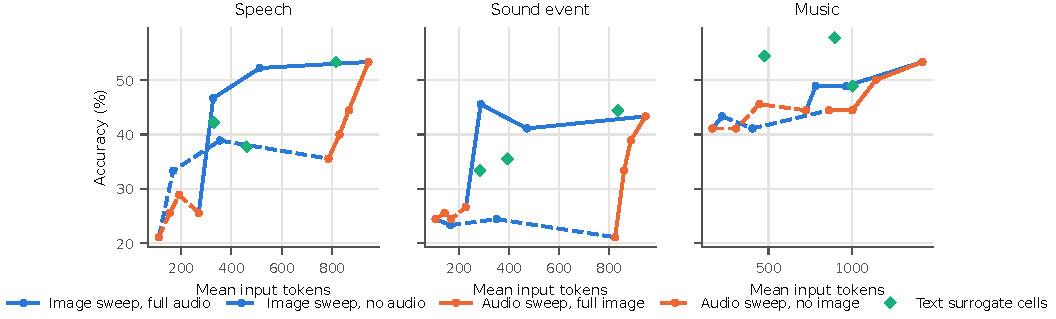
\includegraphics[width=\textwidth]{figures/idea3_marginal_curves_test.pdf}
\caption{Test accuracy vs.\ mean input tokens along each budget sweep. Blue:
image budget $0\!\to\!64\!\to\!256\!\to\!768$ tokens with full (solid) or no
(dashed) audio; orange: audio fraction $0\!\to\!\tfrac14\!\to\!\tfrac12\!\to\!1$
with full (solid) or no (dashed) image. Most of the image's value arrives in the
first 64 tokens, and only when audio is present.}
\label{fig:idea3-curves}
\end{figure*}

\paragraph{Image tokens saturate early.} The marginal utility of visual tokens
is concentrated in the first 64 (\cref{tab:idea3-grid,fig:idea3-curves}). With
full audio, a 64-token image reaches 47.0\% on test vs.\ 50.0\% for the
768-token image (paired difference $-3.0$, bootstrap 95\% CI $[-8.5,2.6]$) at
42\% of the input tokens; on dev the gap is $-0.7$ $[-7.0,5.2]$. Going from no
image to 64 tokens, by contrast, adds $+14.8$ points on test ($[7.0,23.0]$).
Audio length matters less than expected: keeping the first half of the clip
is indistinguishable from the full clip (audio only: $-0.7$ dev, $+0.7$ test).

\begin{figure}[t]
\centering
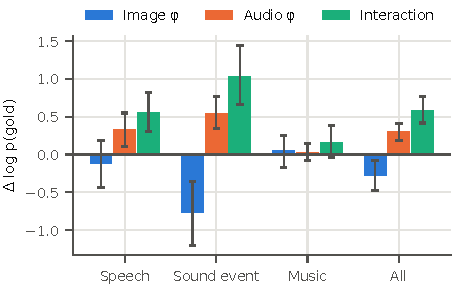
\includegraphics[width=\columnwidth]{figures/idea3_shapley.pdf}
\caption{Per-item Shapley values and interaction on $s=\log p(\text{gold})$,
dev and test pooled ($n{=}180$; bootstrap 95\% CI). Alone, the image
\emph{lowers} the gold-answer probability on sound events; together with audio,
the two modalities are strongly super-additive.}
\label{fig:idea3-shapley}
\end{figure}

\paragraph{Contributions are not additive.} \Cref{fig:idea3-shapley} shows
the attribution. On sound events the image's Shapley value is negative on
both splits (test $\phi_v=-0.74$ $[-1.38,-0.10]$; dev $-0.79$
$[-1.37,-0.25]$), audio's is positive (test $+0.52$ $[0.23,0.85]$), and the
interaction is large (test $I=+1.28$ $[0.73,1.88]$; all types $+0.60$
$[0.36,0.85]$, dev $+0.57$). The image alone does not merely fail to help: it
makes the model \emph{confidently wrong}. With image only, 36\% (dev) and 37\%
(test) of sound-event predictions are wrong with probability $>0.9$, vs.\
10--13\% with audio only. Because $I\gg0$, the utility of image tokens
depends on whether audio is present, so budgets cannot be chosen one modality
at a time. This finding replicates on held-out data; the accuracy-level
patterns we reported in Assignment~2 (e.g.\ ``audio alone beats image alone on
sound events'') hold on test as well, but other accuracy differences flip
between splits.

\begin{table}[t]
\caption{Budget policies selected on dev and scored on test. Cost is input
tokens relative to the full input. Per-type policies pick one cell per audio
type.}
\label{tab:idea3-policies}
\centering\small
\setlength{\tabcolsep}{3pt}
\begin{tabular}{llcc}
\toprule
Policy & Cells (speech / sound / music) & Acc. & Cost \\
\midrule
Always ``D''         & --                                 & 25.2 & -- \\
Full input           & $(768,1)$                          & 50.0 & 1.00 \\
Global, $\beta{=}.4$ & $(64,1)$                           & 47.0 & 0.40 \\
Per type, $\beta{=}.4$ & $(0,1)$ / $(64,1)$ / $(256,0)$    & 37.4 & 0.29 \\
Per type, $\beta{=}.6$ & $(256,1)$ / $(64,1)$ / $(256,0)$  & 46.3 & 0.38 \\
\, + surrogates, $\beta{=}.6$ & $(256,1)$ / $(64,1)$ / Cap+Tr & 50.7 & 0.40 \\
\, + surrogates, $\beta{=}.8$ & $(256,1)$ / $(64,1)$ / Img+Tr & 51.9 & 0.50 \\
Oracle (robust)      & per item                           & 52.2 & 0.22 \\
\bottomrule
\end{tabular}
\end{table}

\paragraph{Per-audio-type allocation overfits.} The premise of the baseline
is that the best cell depends on audio type. \Cref{tab:idea3-policies} shows
that a per-type table chosen on dev does \emph{worse} on test than one global
cell at the same budget: at $\beta=0.4$ it scores 37.4\% vs.\ 47.0\%
($-9.6$, $[-14.8,-4.8]$). Its music choice, image only at 256 tokens, was
the best music cell on dev (57.8\%) but scores 41.1\% on test, and its speech
choice drops the image entirely. The per-type accuracy surfaces are only
weakly stable across splits: the Spearman correlation of the 19 cell
accuracies between dev and test is 0.39--0.51 within each audio type and 0.57
overall. Thirty items per type are too few to rank 19 cells. Adding text
surrogates as candidates helps (50.7\% at 40\% cost; 51.9\% at 50\%, $+1.9$
$[-1.9,5.9]$ over the full input), mainly because image+transcript is the
strongest cell overall. The robust oracle reaches 52.2\% at 22\% of the cost,
so the remaining headroom lies in cost, not accuracy, and it is item-level, not
type-level.

\paragraph{Failure analysis.} Sorting items by the effect of adding the
image to the audio ($s_{va}-s_a$), the 25 worst items are 16 sound events, 7
speech and 2 music, mostly \emph{Action and Activity} and \emph{Story
Description} questions. They share one structure: the image shows a static
scene that matches a distractor, and only the audio reveals the event. In
item 736 (\emph{``What is this man doing?''}; audio: mechanical clicking;
image: a man holding handcuffs), audio alone puts 0.52 on the correct
\emph{``Using handcuffs''}, but the image moves 0.99 of the mass to
\emph{``Showcasing handcuffs''}, and adding the audio back leaves it at 0.99:
the image overrides the audio. In item 726 the options factor as
\{police car, fire truck\}$\times$\{honking, in motion\}. The image settles
the vehicle and the audio settles the action, but the model takes the
visually implied action (\emph{``fire truck is in motion''}). In item 842 a
cartoon dragon is drawn mid-flight while the audio is a startled scream; the
model picks \emph{``flying happily''} over \emph{``didn't fly, it fell
down''}. These are failures of cross-modal composition: the model resolves
each factor from the most salient modality instead of combining evidence. This
matches the visual dominance and modality imbalance reported for jointly
trained multimodal models~\citep{wu2022greedy,peng2022ogm}. A second, smaller
failure mode concerns truncation. We expected a centered window to preserve
short sound events better than the leading segment, but it is slightly worse
(25\%: $-1.9$, 50\%: $-3.7$ points, n.s.). Sound-event clips are short (median
3.4\,s), so the 1\,s floor makes the 25\% and 50\% cells nearly identical, and
truncation is not where the budget is lost.

\subsection{Updated Research Idea}

The midterm results change Idea~3 in three ways. (i) The relevant decision is
\emph{whether} to include a modality and at roughly what resolution, not a
fine-grained token count: 64 visual tokens and half the audio retain nearly
all of the measured utility. (ii) Audio type is too coarse a signal, and a
lookup table over it overfits; the oracle headroom is item-level. (iii)
Because $I(x)\gg0$ and the image induces confident errors, the allocator must
reason jointly about modalities and must not trust the confidence of a
single-modality pass.

For the final report we will replace the lookup table with an
\textbf{interaction-aware item-level allocator}. A cheap first pass at
$b_0=(64,\tfrac12)$ (about 30\% of the full cost) produces features
$z(x)$: the option distribution, the two disagreement statistics
$\mathrm{KL}(p_{v}\,\|\,p_{a})$ and $\mathrm{KL}(p_{va}\,\|\,p_{a})$ computed
from low-budget single-modality passes, and a question embedding. A small
regressor $g_\psi$ predicts the score gain of each upgrade, and the policy
\begin{equation}
\pi(x)=\arg\max_{b\in\mathcal{B}}\ g_\psi\big(z(x),b\big)-\lambda\,c(x;b)
\end{equation}
is trained by cross-fitting on the dev grid and evaluated on test against
this midterm's global and per-type baselines. The disagreement features target
the failure mode above: when the image and audio point to different options,
the item probably needs compositional fusion, which the full raw input
handles worst and image+transcript handles best. To keep the target from being
dominated by noise, we will train on permutation-robust correctness and
$\log p(\text{gold})$, and we will report interaction estimates under a
partial-information-decomposition view~\citep{liang2023pid} to separate
redundant from synergistic items. As a stronger point of comparison for the
resolution axis, we will also test attention-based visual token pruning in
the style of FastV~\citep{chen2024fastv} and nested visual
tokens~\citep{cai2024matryoshka} in place of resizing the image.
